\documentclass{article}

\usepackage[T1]{fontenc} 
\usepackage[utf8]{inputenc}
\usepackage[polish]{babel}




\renewcommand{\contentsname} {Spis treści}

\usepackage{graphicx}

\begin{document}
 
\begin{titlepage} 
	\newcommand{\HRule}{\rule{\linewidth}{0.5mm}} 
	
	\center 
	
	\textsc{\LARGE POLITECHNIKA WROCŁAWSKA WYDZIAŁ ELEKTRONIKI}
	
	\HRule\\[3.0cm]
	
	{\huge Projekt z rozproszonych i obiektowych systemów baz danych}\\[2.0cm] 
	
	{\huge\bfseries Rozproszony system bazodanowy przeznaczony do obsługi oddziałów restauracji}\\[2.0cm] 
	
	
	

	\begin{minipage}{0.4\textwidth}
		\begin{flushleft}
			\large
			\textit{AUTORZY}\\
			Michał Kalinowski\\
			Paweł Kolak\\
			Dawid Mikowski\\
		\end{flushleft}
	\end{minipage}
	~
	\begin{minipage}{0.4\textwidth}
		\begin{flushright}
			\large
			\textit{PROWADZĄCY ZAJĘCIA}\\
			Dr inż. Robert Wójcik
			\\[2.0cm] 
			OCENA PRACY:
		\end{flushright}
	\end{minipage}
	
	% If you don't want a supervisor, uncomment the two lines below and comment the code above
	%{\large\textit{Author}}\\
	%John \textsc{Smith} % Your name
	
	%------------------------------------------------
	%	Date
	%------------------------------------------------
	
	\vfill\vfill\vfill % Position the date 3/4 down the remaining page
	\HRule\\[0.5cm]
	{\large\today} % Date, change the \today to a set date if you want to be precise
	
	%------------------------------------------------
	%	Logo
	%------------------------------------------------
	
	%\vfill\vfill
	%\includegraphics[width=0.2\textwidth]{placeholder.jpg}\\[1cm] % Include a department/university logo - this will require the graphicx package
	 
	%----------------------------------------------------------------------------------------
	
	\vfill % Push the date up 1/4 of the remaining page
	
\end{titlepage}
\clearpage

\tableofcontents
 \newpage
\section{Wstęp}
	\subsection{Cele projektu jest}
	Projekt ma na celu zaprojektowanie oraz implementację aplikacji umożliwiającej dostęp do rozproszonej bazy danych sieci restauracji, oraz konfigurację tejże bazy danych. Projekt zakłada wykorzystanie rozproszonej bazy danych celem zwiększenia wydajności systemu. Baza danych stworzona w ramach projektu ma być zlokalizowana na trzech serwerach bazodanowych. Dane będą replikowane od serwera głównego do serwerów klienckich. Użytkownicy będą mieli dostęp do bazy danych restauracji za pośrednictwem dwóch typów aplikacji: klienckiej i administracyjnej.
	
	\subsection{Zakres projektu}
	\paragraph{}
	Zadania projektowe podzielone zostały na trzy rozłączne obszary tematyczne. Pierwszy z nich dotyczył czynności związanych z bazą danych. Została stworzona i skonfigurowana rozproszona baza danych przy pomocy SQL Server firmy Microsoft. Baza znalazł się w trzech odrębnych instancjach sql serwera. Zaprojektowany został fizyczny model bazy oraz dane początkowe. Zrealizowana została replikacja transakcyjna typu master - salve do dwóch serwerów klienckich. Wykonane zostały również testy funkcjonalne replikacji oraz testy wydajnościowe. Baza danych przechowuje tabele opisujące takie dane jak restauracje, lokacje, menu, dania i promocje. Każdy z trzech serwerów zawsze zawiera ten sam zestaw danych co pozostałe serwery. Zmiana dokonana na głównym serwerze widoczne są równocześnie na wszystkich serwerach.
	\paragraph{}
	Kolejnym obszarem była warstwa logiki biznesowej która dotyczy wykonywania operacji na bazie danych. Projekt zakłada zaimplementowanie aplikacji serwerowej opartej o .Net Core oraz web API.  W ramach projektu skonfigurowano serwer IIS oraz połączenie aplikacji z bazą danych. 
	\paragraph{}
	Ostatni zbiór zadań projektowych dotyczył umożliwienia użytkownikowi interakcji z systemem. Projekt zakładał stworzenie interfejsu użytkownika. Obszar ten w naszym przypadku został podzielony na dwie aplikacje. Jedna której zadaniem będzie obsługa klienta w restauracji, głównym zadaniem tej aplikacji będzie wyświetlanie menu. Drugą aplikacją będzie aplikacja administratorska która umożliwi modyfikację danych w bazie. Aplikacje dynamicznie pobiera dane z serwera oraz wykonuje operacje na bazie danych za pośrednictwem interfejsu udostępnionego przez aplikację serwerową. Tą część zrealizowaliśmy przy pomocy technologii Angular. 
	

	\subsection{Architektura systemu}  
	\paragraph{}
	W projekcie jest zrealizowany 3-warstwowy model komunikacji klient/serwer. W modelu tym przetwarzanie danych (funkcje biznesowe) są realizowane po stronie serwera internetowego, zarządzanie danymi - po stronie serwerów baz danych, natomiast po stronie klienta jest realizowana jedynie prezentacja danych z wykorzystaniem przeglądarki internetowej. Dostęp do aplikacji realizującej funkcje biznesowe będzie realizowany poprzez podanie adresu serwera WWW.
	\paragraph{}
	W projekcie wykorzystywane są jednorodne bazy danych (tj. wszystkie bazy danych będą tego samego typu). Dostęp do baz danych realizowany będzie w oparciu o funkcje aplikacji, które komunikują się bezpośrednio z odpowiednimi serwerami bazodanowymi. W warstwie rozproszonej bazy danych zrealizowany zostanie mechanizm umożliwiający replikację informacji pomiędzy węzłami.
	\paragraph{}
	W ramach projektu wykorzystana została replikacja transakcyjna. W tym podejściu istnieje kilka instancji aplikacji oraz serwera bazodanowego, na serwerze master możliwy jest odczyt i zapis, natomiast na pozostałych dwóch serwerach typu slave możliwy jest jedynie odczyt. Prawa do poszczególnych baz dla instancji aplikacji serwerowej zostały tak przydzielone, aby niemożliwy był zapis na serwerach slave, Prawo do zapisu udostępnione jest jedynie użytkownikowi mającemu dostęp do aplikacji administracyjnej, która podłączona jest do głównego serwera bazodanowego.

 
\section{Replikacja w systemie bazy danych}
	\subsection{Pojęcie replikacji i podstawowe informacje}
	\paragraph{}
\textbf{Replikacja danych} – proces powielania informacji pomiędzy różnymi serwerami baz danych. Można rozróżnić następujące rodzaje replikacji:
	\begin{itemize}
	
\item	Replikacja migawkowa (ang. snapshot replication) – rozprowadzane dane mają stan z pewnego określonego momentu w czasie. Ten rodzaj replikacji znajduje głównie zastosowanie przy danych, które nie są często modyfikowane, jednak modyfikacje te mogą być znaczne. Zmiany pomiędzy kolejnymi wykonywanymi migawkami nie są monitorowane.
\item	Replikacja transakcyjna lub przyrostowa (ang. transaction replication) – dane rozprowadzane są na podstawie logów transakcji, dane modyfikowane są tylko na głównym serwerze.
\item	Replikacja dwukierunkowa lub łącząca (ang. merge replication) – dwukierunkowe rozprowadzanie danych; serwer realizuje transakcje zarówno od innego serwera, jak i od klientów. Transakcje realizowane przez klientów mogą być również przeprowadzone bez połączenia pomiędzy serwerami, jednak w takim przypadku w czasie synchronizacji może dojść do konfliktu, który musi być rozwiązany przez osobę przeprowadzającą aktualizację.

	\end{itemize}

Replikacja w SQL Serwerze oparta jest na technice publikacji i subskrypcji danych. Serwer udostępniający dane jest publikatorem danych. Przesyła on kopie wszystkich zmian opublikowanych danych do serwera zajmującego się dystrybucja, tzw. dystrybutora.
Dystrybutor zawiera bazę dystrybucji, która otrzymuje wszelkie zmiany wprowadzane w danych, przechowuje je i przesyła do serwerów subskrypcji (subskrybentów), obsługujących bazę docelową, która odbiera opublikowane dane i przechowuje ich kopię.
Subskrybent może pobierać wszystkie dane publikowane przez serwer źródłowy lub tylko ich część. Serwer dystrybucji i publikator mogą być na tym samym komputerze lub na innych.

\paragraph{}
Komponenty replikacji są następujące:
	\begin{itemize}
\item	\textbf{Publikator} – serwer udostępniający dane innym serwerom. Przechowuje dane o wszystkich publikacjach dokonanych w bazie danych.
\item	\textbf{Dystrybutor} – serwer zawierający bazę zarządzającą dystrybucją danych
\item	\textbf{Subskrybent} - serwer przechowujący kopie publikacji i przesyłający lub odbierający zmiany od publikatora. Może być również publikatorem dla innych subskrybentów.
\item	\textbf{Artykuł} – zbiór danych, który ma być replikowany i może zawierać dane przechowywanej procedury lub tablicy przeznaczonej do replikacji.
\item	\textbf{Publikacja} – zbiór jednego lub wielu artykułów. Subskrybenty subskrybują publikacje, a nie artykuły.
10
\item \textbf{Subskrybcja} – tworzona jest w celu pobrania publikacji przeznaczonych do replikacji

\end{itemize}

\paragraph{}
Replikacja transakcyjna opiera się w głównej mierze na tzw. agentach. Są to exe'ki, które mogą być uruchamiane z wiersza poleceń, aczkolwiek w większości scenariuszy uruchamia je SQL Server Agent za pomocą Jobów. Poniżej znajduje się lista agentów biorących udział w opisywanym rodzaju replikacji transakcyjnej. Lista ta nie uwzględnia wszystkich agentów związanych z replikacją w MS SQL Server.
\begin{itemize}
\paragraph{}
\item 
Log Reader Agent - agent (logread.exe) który jest odpowiedzialny za cykliczne odczytywanie logu transakcyjnego publikacyjnej bazy danych w poszukiwaniu transakcji przeznaczonych do replikacji i przekazywaniu ich do Dystrybutora.
Snapshot Agent - agent (snapshot.exe) odpowiedzialny za generowanie snapshotów obiektów bazy publikacyjnej ( jest np. wykorzystywany przy inicjalizowaniu subskrypcji ze snapshotów).
\paragraph{}
\item
Agent Dystrybucji (Distribution Agent) - agent (distrib.exe) odpowiedzialny za aplikowanie replikowanych transakcji oraz snapshotów do tabel subskrybenta. Zródłem danych dla agenta jest baza dystrybucyjna. Agent może być uruchamiany na subskrybencie (Pull Subscription) albo na dystrybutorze (Push Subscription).
\end{itemize}

	\subsection{Replikacja transakcyjna}

	\subsection{Replikacja master-slave}

\section{Model konceptualny i fizyczny bazy danych}
	\subsection{Model konceptualny}

	\subsection{Model fizyczny}

\section{Implementacja bazy danych w środowisku ...}
	\subsection{Realizacja bazy danych}
	\newpage
	\subsection{Definiowanie łączników}
	\newpage
	\subsection{Wykorzystanie mechanizmów replikacji transakcyjnej}
	\newpage
	\subsection{Wykorzystanie mechanizmów replikacji master-slave}
	\newpage
\section{Projekt i implementacja aplikacji}
			\begin{figure}[hbt!]
				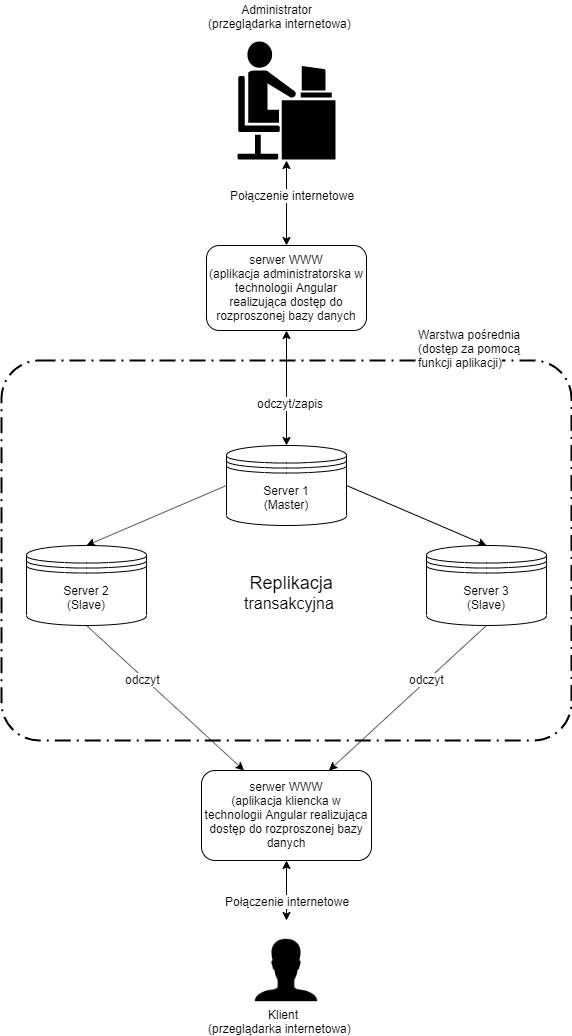
\includegraphics[width=8cm]{Files/Pictures/SystemStruct}
				\centering
				\caption{Diagram przypadków użycia}
			\end{figure}
			\newpage
	\subsection{Aplikacja (Backend)}
	\newpage
	\subsection{Aplikacja (Frontend - Adnin)}
		\subsubsection{Funkcje aplikacji - diagram przypadków użycia}
		Na poniższym rysunku przedstawiono diagram przypadków użycia stworzonej aplikacji administratorskiej. Wszystkie przedstawione na diagramie funkcjonalności zostały zaimplementowane. Ze wsględu na cel projektu głównym celem było przedstawienie możliwości replikacji.
			\begin{figure}[hbt!]
				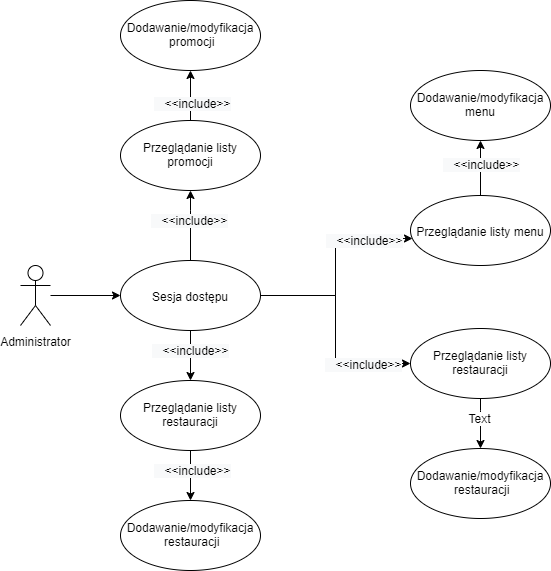
\includegraphics[width=8cm]{Files/Pictures/UMLAdminApp}
				\centering
				\caption{Diagram przypadków użycia}
			\end{figure}
		\subsubsection{Realizacja wybranych funkcjonalności}
		Aplikacja kliencka została zrealizowana w technologi internetowej z wykorzystaniem framework'u Angular 8.
	\subsection{Aplikacja (Frontend - Customer)}
		\subsubsection{Funkcje aplikacji - diagram przypadków użycia}
		Na poniższym rysunku przedstawiono diagram przypadków użycia stworzonej aplikacji klienckiej. Podobnie jak w poprzedniej aplikacji zostały zaimplementowane wszystkie funkcjonalności.
			\begin{figure}[hbt!]
				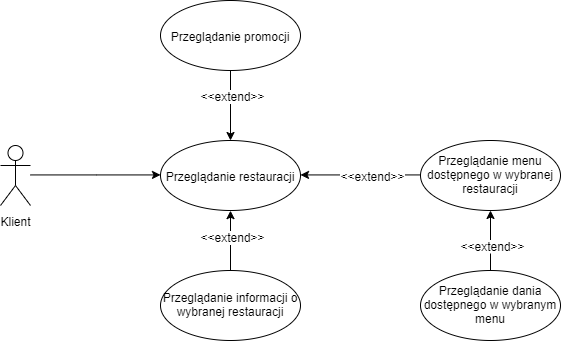
\includegraphics[width=8cm]{Files/Pictures/UMLCustomerApp}
				\centering
				\caption{Diagram przypadków użycia}
			\end{figure}
		\subsubsection{Realizacja wybranych funkcjonalności}	
		Aplikacja kliencka została zrealizowana w technologi internetowej z wykorzystaniem framework'u Angular 8.
\section{Wdrożenie i testowanie aplikacji}

\section{Podsumowanie}

 
1
 
\end{document}